% Options for packages loaded elsewhere
\PassOptionsToPackage{unicode}{hyperref}
\PassOptionsToPackage{hyphens}{url}
\PassOptionsToPackage{dvipsnames,svgnames,x11names}{xcolor}
%
\documentclass[
  letterpaper,
  DIV=11,
  numbers=noendperiod]{scrartcl}

\usepackage{amsmath,amssymb}
\usepackage{lmodern}
\usepackage{iftex}
\ifPDFTeX
  \usepackage[T1]{fontenc}
  \usepackage[utf8]{inputenc}
  \usepackage{textcomp} % provide euro and other symbols
\else % if luatex or xetex
  \usepackage{unicode-math}
  \defaultfontfeatures{Scale=MatchLowercase}
  \defaultfontfeatures[\rmfamily]{Ligatures=TeX,Scale=1}
\fi
% Use upquote if available, for straight quotes in verbatim environments
\IfFileExists{upquote.sty}{\usepackage{upquote}}{}
\IfFileExists{microtype.sty}{% use microtype if available
  \usepackage[]{microtype}
  \UseMicrotypeSet[protrusion]{basicmath} % disable protrusion for tt fonts
}{}
\makeatletter
\@ifundefined{KOMAClassName}{% if non-KOMA class
  \IfFileExists{parskip.sty}{%
    \usepackage{parskip}
  }{% else
    \setlength{\parindent}{0pt}
    \setlength{\parskip}{6pt plus 2pt minus 1pt}}
}{% if KOMA class
  \KOMAoptions{parskip=half}}
\makeatother
\usepackage{xcolor}
\usepackage[left=1in,right=1in,headheight=5mm]{geometry}
\setlength{\emergencystretch}{3em} % prevent overfull lines
\setcounter{secnumdepth}{-\maxdimen} % remove section numbering
% Make \paragraph and \subparagraph free-standing
\ifx\paragraph\undefined\else
  \let\oldparagraph\paragraph
  \renewcommand{\paragraph}[1]{\oldparagraph{#1}\mbox{}}
\fi
\ifx\subparagraph\undefined\else
  \let\oldsubparagraph\subparagraph
  \renewcommand{\subparagraph}[1]{\oldsubparagraph{#1}\mbox{}}
\fi


\providecommand{\tightlist}{%
  \setlength{\itemsep}{0pt}\setlength{\parskip}{0pt}}\usepackage{longtable,booktabs,array}
\usepackage{calc} % for calculating minipage widths
% Correct order of tables after \paragraph or \subparagraph
\usepackage{etoolbox}
\makeatletter
\patchcmd\longtable{\par}{\if@noskipsec\mbox{}\fi\par}{}{}
\makeatother
% Allow footnotes in longtable head/foot
\IfFileExists{footnotehyper.sty}{\usepackage{footnotehyper}}{\usepackage{footnote}}
\makesavenoteenv{longtable}
\usepackage{graphicx}
\makeatletter
\def\maxwidth{\ifdim\Gin@nat@width>\linewidth\linewidth\else\Gin@nat@width\fi}
\def\maxheight{\ifdim\Gin@nat@height>\textheight\textheight\else\Gin@nat@height\fi}
\makeatother
% Scale images if necessary, so that they will not overflow the page
% margins by default, and it is still possible to overwrite the defaults
% using explicit options in \includegraphics[width, height, ...]{}
\setkeys{Gin}{width=\maxwidth,height=\maxheight,keepaspectratio}
% Set default figure placement to htbp
\makeatletter
\def\fps@figure{htbp}
\makeatother

\setkomafont{author}{\small}
\setkomafont{date}{\small}
\KOMAoption{captions}{tableheading}
\makeatletter
\makeatother
\makeatletter
\makeatother
\makeatletter
\@ifpackageloaded{caption}{}{\usepackage{caption}}
\AtBeginDocument{%
\ifdefined\contentsname
  \renewcommand*\contentsname{Table of contents}
\else
  \newcommand\contentsname{Table of contents}
\fi
\ifdefined\listfigurename
  \renewcommand*\listfigurename{List of Figures}
\else
  \newcommand\listfigurename{List of Figures}
\fi
\ifdefined\listtablename
  \renewcommand*\listtablename{List of Tables}
\else
  \newcommand\listtablename{List of Tables}
\fi
\ifdefined\figurename
  \renewcommand*\figurename{Figure}
\else
  \newcommand\figurename{Figure}
\fi
\ifdefined\tablename
  \renewcommand*\tablename{Table}
\else
  \newcommand\tablename{Table}
\fi
}
\@ifpackageloaded{float}{}{\usepackage{float}}
\floatstyle{ruled}
\@ifundefined{c@chapter}{\newfloat{codelisting}{h}{lop}}{\newfloat{codelisting}{h}{lop}[chapter]}
\floatname{codelisting}{Listing}
\newcommand*\listoflistings{\listof{codelisting}{List of Listings}}
\makeatother
\makeatletter
\@ifpackageloaded{caption}{}{\usepackage{caption}}
\@ifpackageloaded{subcaption}{}{\usepackage{subcaption}}
\makeatother
\makeatletter
\@ifpackageloaded{tcolorbox}{}{\usepackage[many]{tcolorbox}}
\makeatother
\makeatletter
\@ifundefined{shadecolor}{\definecolor{shadecolor}{rgb}{.97, .97, .97}}
\makeatother
\makeatletter
\makeatother
\ifLuaTeX
  \usepackage{selnolig}  % disable illegal ligatures
\fi
\IfFileExists{bookmark.sty}{\usepackage{bookmark}}{\usepackage{hyperref}}
\IfFileExists{xurl.sty}{\usepackage{xurl}}{} % add URL line breaks if available
\urlstyle{same} % disable monospaced font for URLs
\hypersetup{
  pdftitle={Study design},
  pdfauthor={Practice problems},
  colorlinks=true,
  linkcolor={blue},
  filecolor={Maroon},
  citecolor={Blue},
  urlcolor={Blue},
  pdfcreator={LaTeX via pandoc}}

\title{Study design}
\author{Practice problems}
\date{9/11/24}

\begin{document}
\maketitle
\ifdefined\Shaded\renewenvironment{Shaded}{\begin{tcolorbox}[frame hidden, sharp corners, boxrule=0pt, borderline west={3pt}{0pt}{shadecolor}, breakable, interior hidden, enhanced]}{\end{tcolorbox}}\fi

Please work on the practice problems in your group. At least one of the
following problems will be assigned to the weekly problem set.

\begin{enumerate}
\def\labelenumi{\arabic{enumi}.}
\item
  In Spring 2024, Prof.~Tang asked her STAT 311 students to fill out a
  mid-semester survey. She was particularly interested in the the amount
  of hours her STAT 311 students were spending per week on the course.
  The average time spent on the course was found to be 10.2 hours per
  week.

  \begin{enumerate}
  \def\labelenumii{\alph{enumii}.}
  \tightlist
  \item
    Based on this information, identify each of the following:
    observation, variable, parameter, and statistic.
  \item
    Was this survey a census or (just) a sample? Why?
  \end{enumerate}
\item
  Time to implement the sampling methods we learned! \textbf{Keep track
  of your work on this problem; we will return to it in the next few
  classes.}

  We have a farmer who grows sunflowers for making sunflower oil. Her
  field is arranged in a grid pattern, with 12 rows and 12 columns as
  shown below. Water is important for crops, so irrigation ditches have
  been installed along the top and bottom of the field. It is expected
  that plants closer to a water source will perform better than those
  further away from water.

  The farmer would like to estimate the number of healthy plants in the
  field, along with a few other characteristics about the sunflowers. It
  would be unfeasible to conduct a census, so we should choose to sample
  a subset of the grid cells. Suppose we'd like to sample \(n = 12\)
  grid cells total.

  \begin{enumerate}
  \def\labelenumii{\alph{enumii}.}
  \item
    Using words (sentences or bulleted list are fine) and perhaps
    labeling the figure below, describe exactly how you would obtain a
    sample of 12 grid cells using \textbf{simple random sampling}. I
    should be able to read your work and know what to do without any
    questions! Think about how you will perform the random sampling.

    Then implement the method that you've written down, and either using
    the figure below or drawing your own 12x12 field, shade in the
    squares that correspond to your sample.

    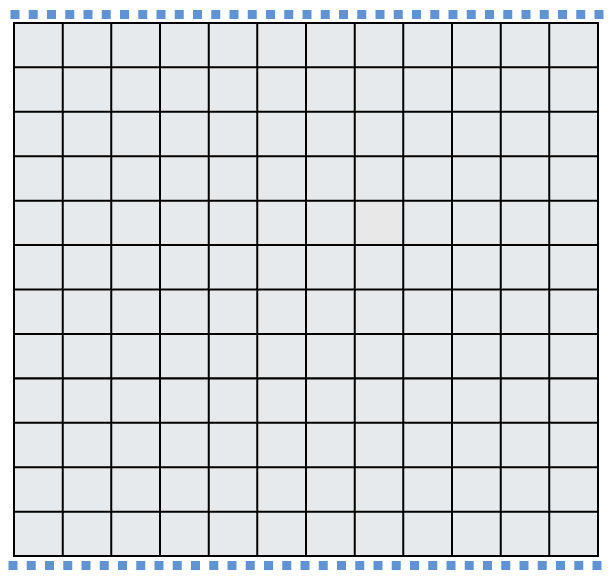
\includegraphics[width=2.22917in,height=\textheight]{figs/sunflower_field.png}
  \item
    Using words (sentences or bulleted list are fine) and perhaps
    labeling the figure below, describe exactly how you would obtain a
    sample of 12 grid cells using \textbf{stratified sampling} where the
    strata are rows. I should be able to read your work and know what to
    do without any questions!

    Then implement the method that you've written down, and either using
    the figure below or drawing your own 12x12 field, shade in the
    squares that correspond to your sample.

    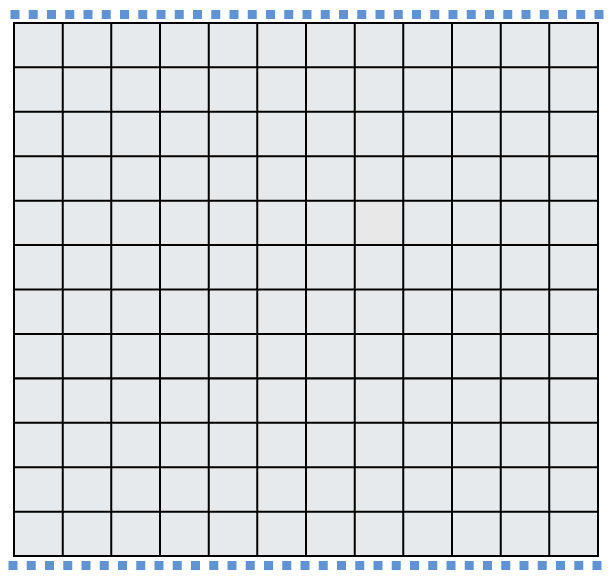
\includegraphics[width=2.22917in,height=\textheight]{figs/sunflower_field.png}
  \item
    Using words (sentences or bulleted list are fine) and perhaps
    labeling the figure below, describe exactly how you would obtain a
    sample of 12 grid cells using \textbf{stratified sampling} where the
    strata are columns. I should be able to read your work and know what
    to do without any questions!

    Then implement the method that you've written down, and either using
    the figure below or drawing your own 12x12 field, shade in the
    squares that correspond to your sample.

    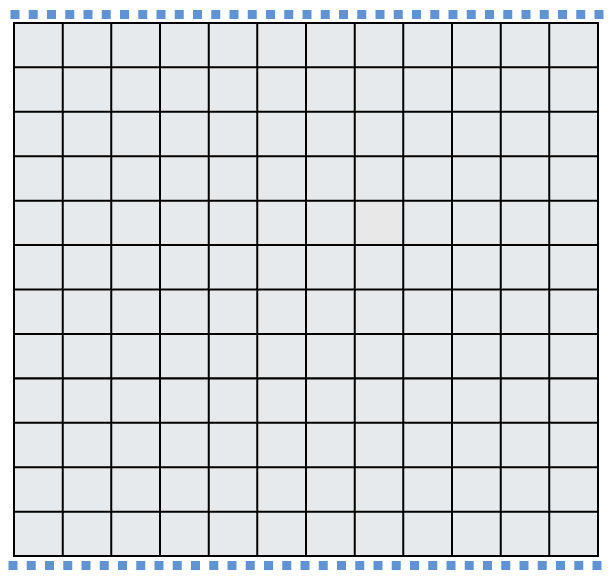
\includegraphics[width=2.22917in,height=\textheight]{figs/sunflower_field.png}
  \item
    Using words (sentences or bulleted list are fine) and perhaps
    labeling the figure below, describe exactly how you would obtain a
    sample of 12 grid cells using \textbf{cluster sampling} where we
    have 24 clusters total. I should be able to read your work and know
    what to do without any questions!

    Then implement the method that you've written down, and either using
    the figure below or drawing your own 12x12 field, shade in the
    squares that correspond to your sample.

    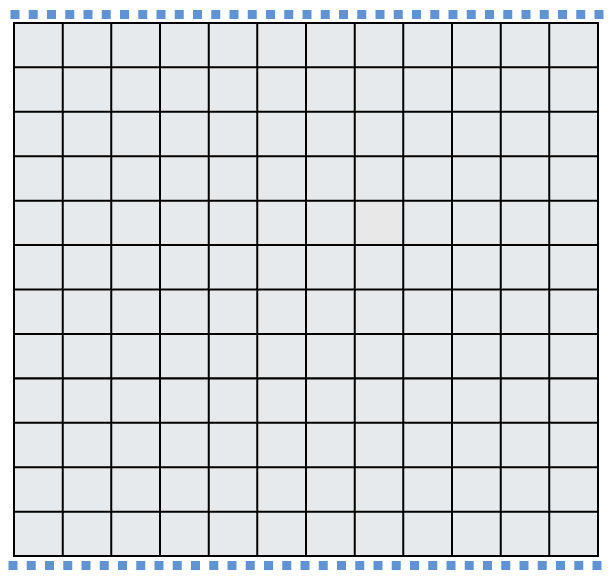
\includegraphics[width=2.22917in,height=\textheight]{figs/sunflower_field.png}
  \item
    Using words (sentences or bulleted list are fine) and perhaps
    labeling the figure below, describe exactly how you would obtain a
    sample of 12 grid cells using \textbf{multistage sampling}. I should
    be able to read your work and know what to do without any questions!

    Then implement the method that you've written down, and either using
    the figure below or drawing your own 12x12 field, shade in the
    squares that correspond to your sample.

    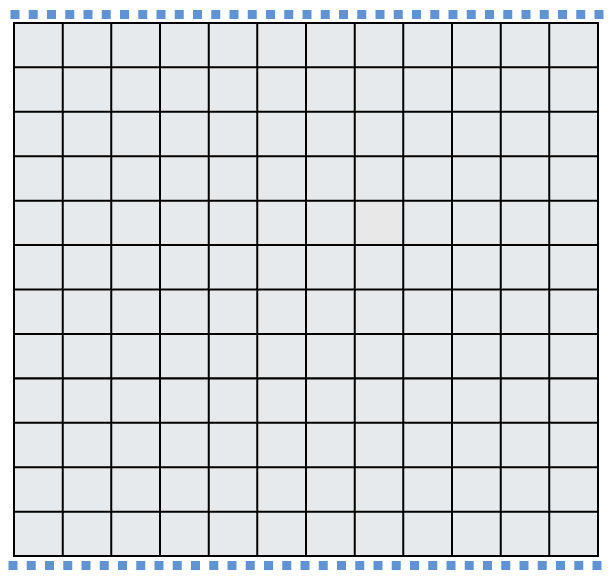
\includegraphics[width=2.22917in,height=\textheight]{figs/sunflower_field.png}
  \end{enumerate}
\item
  Suppose we want to estimate household size, where a
  \emph{``household''} is defined as people living together in the same
  dwelling, and sharing living accommodations. If we select students at
  random at an elementary school and ask them what their family size is,
  will this be a good measure of household size? Or will our average be
  biased? If so, will it overestimate or underestimate the true value?
\item
  To assess the effectiveness of taking large doses of vitamin C in
  reducing the duration of the common cold, researchers recruited 400
  healthy volunteers from staff and students at a university. A quarter
  of the patients were assigned a placebo, and the rest were evenly
  divided between 1g Vitamin C, 3g Vitamin C, or 3g Vitamin C plus
  additives to be taken at onset of a cold for the following two days.
  All tablets had identical appearance and packaging. The nurses who
  handed the prescribed pills to the patients knew which patient
  received which treatment, but the researchers assessing the patients
  when they were sick did not. No statistically discernible differences
  were observed in any measure of cold duration or severity between the
  four groups, and the placebo group had the shortest duration of
  symptoms.

  \begin{enumerate}
  \def\labelenumii{\alph{enumii}.}
  \tightlist
  \item
    Was this an experiment or an observational study? Why?
  \item
    What are the explanatory and response variables in this study?
  \item
    Were the patients blinded to their treatment?
  \item
    Was this study double-blind?
  \item
    Participants are ultimately able to choose whether to use the pills
    prescribed to them. We might expect that not all of them will adhere
    and take their pills. Does this introduce a confounding variable to
    the study? Explain your reasoning.
  \end{enumerate}
\end{enumerate}



\end{document}
